\documentclass[12pt, %
openright,
oneside, %
%twoside, %TCC: Se seu texto tem mais de 100 páginas, descomente esta linha e comente a anterior
a4paper,    %
%english,   %
brazil]{facom-ufu-abntex2}

\usepackage{graphicx}
\usepackage[utf8]{inputenc}
\usepackage[T1]{fontenc}
\usepackage[brazil]{babel}
\usepackage{multirow}
\usepackage{listings}
\usepackage{hyperref}
\usepackage{minted} % https://www.sharelatex.com/learn/Code_Highlighting_with_minted
\renewcommand\listingscaption{Exemplo}

\autor{William Johnson dos Santos Okano} %TCC
\data{2018}
\orientador{Prof. Dr. André Ricardo Backes} %TCC
%\coorientador{Algum?} %TCC


% ---
% Informações de dados para CAPA e FOLHA DE ROSTO
% ---

\titulo{Implementação de uma biblioteca gráfica multiplataforma utilizando OpenGL e GLFW} %TCC

\hypersetup{pdfkeywords={biblioteca}{opengl}{multiplataforma}{glfw}} %TCC

\begin{document}
\frenchspacing

% ----------------------------------------------------------
% ELEMENTOS PRÉ-TEXTUAIS
% ----------------------------------------------------------
%\pretextual
\imprimircapa
\imprimirfolhaderosto


% ---
% Inserir folha de aprovação
% ---
%
% \includepdf{folhadeaprovacao_final.pdf} %TCC: depois de aprovado o trabalho, descomente esta linha e comente o próximo bloco para incluir scan da folha de aprovação.
%

\begin{folhadeaprovacao}

  \begin{center}
    {\ABNTEXchapterfont\large\imprimirautor}

    \vspace*{\fill}\vspace*{\fill}
    {\ABNTEXchapterfont\bfseries\Large\imprimirtitulo}
    \vspace*{\fill}

    \hspace{.45\textwidth}
    \begin{minipage}{.5\textwidth}
        \imprimirpreambulo
    \end{minipage}%
    \vspace*{\fill}
   \end{center}

   Trabalho aprovado. \imprimirlocal, 20 de Julho de 2018: %TCC:

   \assinatura{\textbf{\imprimirorientador} \\ Orientador}
   \assinatura{\textbf{Prof. Dr. Mauricio Cunha Escarpinati}}% \\ Convidado 1} %TCC:
   \assinatura{\textbf{Prof. Me. William Chaves de Souza Carvalho}}% \\ Convidado 2} %TCC:
   %\assinatura{\textbf{Professor} \\ Convidado 3}
   %\assinatura{\textbf{Professor} \\ Convidado 4}

   \begin{center}
    \vspace*{0.5cm}
    {\large\imprimirlocal}
    \par
    {\large\imprimirdata}
    \vspace*{1cm}
  \end{center}

\end{folhadeaprovacao}

% ---


%%As seções dedicatória, agradecimento e epígrafe não são obrigatórias.
%%Só as mantenha se achar pertinente.

% ---
% Dedicatória
% ---
%\begin{dedicatoria}
%   \vspace*{\fill}
%   \centering
%   \noindent
%   \textit{Dedico a \lipsum[10]}  %TCC:
%   \vspace*{\fill}
%\end{dedicatoria}
% ---

% ---
% Agradecimentos
% ---
\begin{agradecimentos}
Gostaria de agradecer ao meu orientador, Prof. Dr. André Ricardo Backes pela paciência em todos esses semestres. %TCC:
\end{agradecimentos}
% ---

% ---
% Epígrafe
% ---
\begin{epigrafe}
    \vspace*{\fill}
	\begin{flushright}
        \textit{``NO sucesso é a soma de pequenos }\\
        \textit{esforços repetidos dia após dia.''}\\
        (Robert Collier)
	\end{flushright}
\end{epigrafe}
% ---


%\iffalse % Descomentar Resumo no final
\begin{resumo} %TCC:
 A dificuldade de aprendizagem de programação pode ser causada por várias razões, como a incapacidade de compreensão de algoritmos por este ser um conceito muito abstrato.
 
 Várias são as formas utilizadas no ensino de algoritmos e estruturas de controle. Este trabalho apresenta uma proposta de biblioteca para auxiliar o ensino de programação, utilizando conceitos gráficos para facilitar o entendimento das estruturas de programação. A solução proposta tem como foco desenvolver uma biblioteca multiplataforma, com um conjunto de funções simples para gerenciamento de elementos gráficos, bem como a elaboração de um guia de utilização e sua respectiva documentação.

 \vspace{\onelineskip}

 \noindent
 \textbf{Palavras-chave}: Biblioteca de funções, elementos gráficos, OpenGL. %TCC:
\end{resumo}
%\fi

% ---
% inserir lista de ilustrações
% ---
\pdfbookmark[0]{\listfigurename}{lof}
\listoffigures*
\cleardoublepage
% ---

\iffalse
% ---
% inserir lista de tabelas
% ---
\pdfbookmark[0]{\listtablename}{lot}
\listoftables*
\cleardoublepage
% ---
\fi


% ---
% inserir lista de abreviaturas e siglas
% ---
\begin{siglas} %TCC:
  \item[API] \textit{Application Programming Interface}
  \item[FPS] \textit{Frames per second (Quadros por segundo)}
  \item[GLFW] \textit{Graphics Library Framework}
  \item[GLUT] \textit{OpenGL Utility Toolkit}
  \item[IDE] \textit{Integrated Development Environment (Ambiente de Desenvolvimento Integrado)}
  \item[RGB] \textit{Red, Green, and Blue (Vermelho, Verde e Azul)}
  \item[SDL] \textit{Simple DirectMedia Layer}
  \item[TI] \textit{Tecnologia da Informação}
  %\item[456] Isto é um número
  %\item[123] Isto é outro número
  %\item[Zézão] este é o meu nome
\end{siglas}
% ---

%% ---
%% inserir lista de símbolos, se for adequado ao trabalho. %TCC:
%% ---
%\begin{simbolos}
%  \item[$ \Gamma $] Letra grega Gama
%  \item[$ \Lambda $] Lambda
%  \item[$ \zeta $] Letra grega minúscula zeta
%  \item[$ \in $] Pertence
%\end{simbolos}
%% ---

% ---
% inserir o sumario
% ---
\pdfbookmark[0]{\contentsname}{toc}
\tableofcontents*
\cleardoublepage
% ---





% ----------------------------------------------------------
% ELEMENTOS TEXTUAIS
% ----------------------------------------------------------
\textual


% ----------------------------------------------------------
% Introdução
% ----------------------------------------------------------

\chapter[Introdução]{Introdução}
Segundo \cite{de2004ferramenta}, um dos grandes problemas entrentados em muitas intituições de ensino é relacionado ao baixo índice de assimilação dos estudantes nas disciplinas onde o conhecimento de programação seja um requisito. Uma das razões para a dificuldade no aprendizado é que as linguagens de programação possuem entidades muito abstratas, sendo difícil a visualização de como ocorre o fluxo das informações dentro de estruturas de controles, tais como laços de repetição e condicionais lógicas, ponteiros, \textit{arrays}, etc.

Muitos alunos de cursos introdutórios utilizam-se das mais diversas técnicas de aprendizado para tentar assimilar o funcionamento de um programa ou algoritmo. Uma das técnicas é a utilização de fluxogramas, onde são desenhadas caixas, setas e direções de como o programa deve se comportar, ou então a execução passo à passo, onde anota-se o valor de cada variável em cada linha, laço de repetição ou condicional lógica executado. Alguns optam por utilizar ferramentas de auxílio visual, como o \citeonline{Scratch:About} ou \citeonline{RubyWarrior:About}. Apesar de serem excelentes ferramentas de ensino, estas ferramentas apresentam alguns pontos fracos. O Scratch, por exemplo, é uma linguagem de programação própria, enquanto RubyWarrior utiliza a linguagem de programação \citeonline{Ruby:About}. No entanto, em cursos de introdução à programação, geralmente, é utilizada a linguagem de programação C.

Com a introdução e popularização das linguagens \citeonline{CPP:About} e \citeonline{Java:About}, vários programadores optaram por deixar a linguagem de programação C. Apesar de ela ainda ser considerada uma importante linguagem de programação, tanto na indústria da engenharia, quanto nas instituições de ensino, ela carece de ferramentas de visualização. A maioria das ferramentas de visualização de programação feitas para a linguagem C são focadas em algoritmos avançados, como algoritmos de ordenação, grafos, e não nas necessidades de um iniciante em programação, como declaração de variáveis, funções e ponteiros \cite{kirby2010program}.

De acordo com \citeonline{mayer1981psychology}, a aquisição de novo conhecimento pode ser obtido através do relacionamento da nova informação com as informações previamente adquiridas, utilizando as informações antigas como reforço de memória enquanto assimila as novas informações. Segundo \citeonline{souza2000sistema}, um grande motivador do processo de ensino aprendizagem é a utilização de alguma ferramenta computacional que permita os alunos confeccionar os seus algoritmos bem como testarem as suas soluções visualizando o resultado gerado por elas.

\section{Objetivos}
O objetivo geral deste trabalho é a implementação de uma biblioteca gráfica, baseada em OpenGL, que dê a possibilidade aos alunos de cursos introdutórios de programação compreender, de forma visual, os efeitos dos códigos ensinados em sala de aula. Os objetivos específicos do trabalho proposto são:

\begin{enumerate}
\item Criação de uma biblioteca gráfica que seja de fácil instalação;
\item Criação de uma biblioteca que possua uma API simples e objetiva;
\item Criação de um manual de utilização e exemplos da biblioteca.
\end{enumerate}

\section{Funcionalidades previstas}
Apesar de ser uma abstração da biblioteca OpenGL, este trabalho não possui funções para a manipulação de janelas diretamente, com exceção da função que inicializa a biblioteca, na qual é automaticamente criada uma janela e um contexto OpenGL.

As funcionalidades previstas para este trabalho podem ser divididas em 3 categorias: funções de gerenciamento da biblioteca; funções de configuração dos objetos; e funções de desenho.

As funções da biblioteca são divididas da seguinte forma:
\begin{itemize}

    \item Funções de gerenciamento
    \begin{itemize}
    \item Inicializar a biblioteca;
    \item Limpar a tela;
    \item Desfazer o último desenho;
    \item Refazer o último desenho.
    \end{itemize}

    \item Funções de configuração
    \begin{itemize}
    \item Definir a cor de preenchimento do objeto;
    \item Obter a cor de preenchimento do objeto;
    \item Definir o tamanho de um ponto;
    \item Obter o tamanho de um ponto;
    \item Definir a largura de uma linha;
    \item Obter a largura de uma linha.
    \end{itemize}

    \item Funções de desenho
    \begin{itemize}

    \item Polígono;
    \item Ponto;
    \item Triângulo;
    \item Retângulo;
    \item Quadrado;
    \item Polígono regular;
    \item Círculo;
    \item Pentágono;
    \item Hexágono;
    \item Decágono;
    \item Dodecágono;
    \item Linha.

    \end{itemize}
\end{itemize}

\chapter{Trabalhos Correlatos}
Nesta seção serão apresentadas algumas bibliotecas que fazem o gerenciamento de janelas e contexto OpenGL, bem como algumas ferramentas que auxiliam no ensino da programação fazendo uso de técnicas de visualização. Existem várias outras bibliotecas que fazem o gerenciamento de janelas OpenGL, assim como também existem várias outras ferramentas que ensinam programação através da tecnica de visualização, porém, as bibliotecas e ferramentas apresentadas a seguir possuem semelhança com o objetivo deste trabalho.

\section{Borland Graphics Interface}
A biblioteca \textit{Borland Graphics Interface}, também conhecida como BGI, é uma biblioteca gráfica para as linguagens C e C++ que é distribuída junto a vários compiladores da Borland para o sistema operacional DOS \cite{BGI:Drivers}, e eventualmente com suporte a Windows, desde 1987. A biblioteca BGI é menos poderosa que outras bibliotecas, como a SDL ou OpenGL pois foi desenvolvida para a apresentação de gráficos e não para a criação de aplicações 3D baseadas em eventos. Entretanto, ela possui uma API muito simples de ser utilizada e que ajudou na sua popularização. O manual da BGI pode ser encontrado em \citeonline{BGI:Manual}

\section{GLUT e FreeGLUT}
\citeonline{GLUT:About} é o kit de ferramentas utilitárias para o desenvolvimento de programas OpenGL nas linguagens C e C++, utilizando um sistema de gerenciamento de janelas. Este kit de ferramentas faz com que seja consideravelmente mais fácil aprender e explorar a programação utilizando OpenGL. Além do mais, provê uma API portável, permitindo que seja aproveitado o mesmo código OpenGL com GLUT entre vários sistemas operacionais.

Além disso, o GLUT é designado para construir aplicações de pequeno e médio porte já que, apesar de bem adequado tanto para o aprendizado, quanto para o desenvolvimento de aplicações simples usando OpenGL, ele não é um kit com todos os recursos necessários para se escrever aplicações de grande porte.

Já o \citeonline{FreeGLUT:About} é uma versão alternativa de código-aberto à biblioteca GLUT, pois esta possui licença proprietária de autoria de Mark Kilgard. Foi desenvolvida em 1999 e liberada sob a licença \textit{X-Consortium}. A biblioteca FreeGLUT possui todas as funcionalidades da biblioteca GLUT, além de possuir algumas funcionalidades adicionais. Apesar de ser uma alternativa de código-aberto e mais atualizada em relação ao GLUT, ambas as bibliotecas estão defasadas. A última atualização da biblioteca GLUT ocorreu em 1998, com a versão 3.7. Atualmente ela não se econtra mais em desenvolvimento. Já a última atualização da biblioteca FreeGLUT ocorreu em março de 2015, com a versão 3.0.0. A biblioteca FreeGLUT pode ser encontrada em \url{http://freeglut.sourceforge.net/}.

\section{SDL}
\citeonline{SDL:About} (SDL), é uma biblioteca de desenvolvimento multiplataforma desenvolvida para prover acesso de baixo nível nos \textit{hardwares} de áudio, teclado, mouse e \textit{joystick} por meio da OpenGL e Direct3D.

SDL possui código-aberto, sob a licença \citeonline{zliblicence}. Além disso, possui suporte nativo oficial a Windows, Mac OS X, Linux, iOS e Android. Ela é escrita totalmente na linguagem C e possui compatibilidade com C++, além de possuir versões para outras linguagens de programação, como \citeonline{Java:About}, \citeonline{CSharp:About} e \citeonline{Python:About}.

\section{Ferramentas de técnica de visualização}
Atualmente existem diversas ferramentas que auxiliam na aprendizagem utilizando técnicas de visualização. As ferramentas variam entre animações interativas, linguagem de programação visual ou programação de ações de personagens. Abaixo são apresentadas algumas ferramentas que fazem o uso dessa técnica utilizando as características citadas:

\begin{itemize}

    \item \citeonline{Scratch:About}, trata-se de uma linguagem de programação visual onde é possível programar histórias, jogos e animações interativas. Scratch ajuda os jovens a pensar de forma criativa e raciocinar sistematicamente. Por se tratar de linguagem de programação visual, ao invés de escrever linhas de códigos, o usuário arrasta blocos e os conecta, desenvolvendo assim todo o fluxo da aplicação. Foi projetada com foco no público de pessoas entre 8 e 16 anos, mas é utilizada por pessoas de todas as idades.

    \item \citeonline{RubyWarrior:About}, é um jogo onde o usuário, no controle de um guerreiro, deve completar as missões usando a linguagem de programação \citeonline{Ruby:About} como método de controle do personagem;

    \item \citeonline{RaftOnline:About}, é um website que possui uma simulação interativa do funcionamento do algoritmo de consensus Raft. O site permite várias configurações e ações, sendo possível derrubar um nó para observar o comportamento de eleição de novo líder.

\end{itemize}


\chapter{Desenvolvimento}

\section{Tecnologias Empregadas}

\subsection{Linguagem de programação C}\label{lbl:linguagem_programao_c}
A linguagem de programação \citeonline{C:About} foi criada por Dennis MacAlistair Ritchie entre 1969 e 1973 na \citeonline{BellLabs:Site} e trata-se de uma linguagem de propósito geral que pode ser utilizada com os paradigmas imperativo, também conhecido como procedural, e o paradigma estruturado. Segundo o site \citeonline{GeneralPurposeLanguage:About}, uma linguagem de propósito geral é aquela que não é limitada apenas à algum tipo de hardware específico ou para uma aplicação especializada.

A linguagem de programação C foi escolhida por ser uma das linguagens mais utilizadas para o ensino de programação nas universidades brasileiras. Uma pesquisa conduzida online em um grupo de programação chamado A.P.D.A. Associação dos Programadores Depressivos Anônimos, um fórum que concentra mais de 71.000 programadores e entusiastas brasileiros, foi obtido um resultado de que aproximadamente 55\% das universidades brasileiras escolhem C como a primeira, ou uma das primeiras, linguagens para o ensino de introdução à programação, como pode-se observar na Figura ~\ref{fig:pesquisa_linguagem_tcc}. Este dado representa 570 votos em uma pesquisa com 1036 respostas. A linguagem de programação Java, que se ficou em segundo lugar como mais utilizada, teve apenas 169 votos, representando 16,31\% do total de votos. Esse resultado pode ser encontrada no link \url{https://www.facebook.com/groups/osadpa/permalink/1508699765902212/}.

Apesar do nome caricato do grupo onde foi conduzida a pesquisa, trata-se de um grupo sério sobre programação em geral, sendo utilizado por uma vasta gama de profissionais de TI.

\pagebreak
\begin{figure}[htbp]
  \centering
  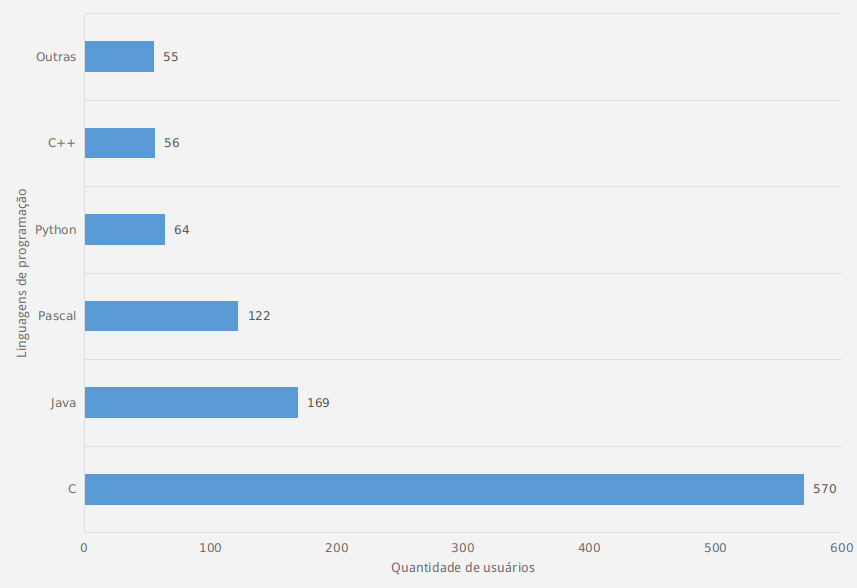
\includegraphics[scale=0.51]{images/pesquisa_linguagem_tcc.png}
  \caption{Linguagens de programação utilizadas primariamente no ensino de introdução à programação}
  \label{fig:pesquisa_linguagem_tcc}
\end{figure}

\subsection{OpenGL}
O \citeonline{OpenGL:About} é uma biblioteca gráfica para desenvolvimento de aplicações interativas. Desde sua introdução, no ano de 1992, a biblioteca OpenGL se tornou a interface de programação de aplicação (API) mais utilizada com suporte a 2D e 3D pela indústria. O OpenGL foi escolhido como biblioteca gráfica por sua qualidade de ser altamente portável estando presente em várias plataformas, tais como Windows, Linux, Unix, MacOS, entre outras. Outro motivo foi o fato de possuir um bom desempenho, e de poder ser utilizada em conjunto com várias linguagens de programação, dentre as quais foi escolhida a linguagem de programação \citeonline{C:About}.

A biblioteca gráfica \citeonline{OpenGL:About} foi escolhida em detrimento de outras por ser mais simples, porém versátil, e suas já citadas qualidades: performance, largamente utilizada, interoperável entre plataformas e por ter fácil integração com a linguagem de programação C. Outros fatores que influenciaram a sua escolha foi a vasta documentação, como websites, livros e cursos online. Alguns sites que promovem a documentação de utilização do OpenGL são o próprio site do OpenGL \url{https://opengl.org/}, o website \citeonline{LearnOpenGL:Site} e o livro OpenGL Programming Guide: The Official Guide to Learning OpenGL, Version 1.2, do autor \citeonline{Woo:1999:OPG:554539}.

A forma que o OpenGL trabalha para renderizar os objetos na tela é baseada em uma máquina de estados. Cada item renderizado pelo OpenGL fica num buffer secundário e só é renderizado quando explicitamente solicitado. Ao renderizar o buffer ele então faz a troca do buffer primário pelo secundário, exibindo assim apenas o quadro renderizado por completo, evitando assim o \textit{tearing}. \textit{Tearing} é o efeito que ocorre quando parte do frame é renderizado utilizando informações antiga, exibindo assim parte do quadro com uma imagem e outra parte com os dados novos.

\subsection{GLFW}
De acordo com o site da \citeonline{GLFW:About}, GLFW é uma biblioteca gráfica de código-aberto, multiplataforma para desenvolvimento desktop, que utiliza OpenGL, OpenGL ES e Vulkan. Ela é responsável por criar janelas de forma unificada entre diferentes sistemas operacionais, contextos OpenGL e receber entradas de dados e eventos.

A biblioteca GLFW foi escrita em C e possui suporte nativo para Windows, macOS e vários sistemas Unix \cite{Unix:About} que utilizam o sistema de janelas X Window System \cite{X:About}, como por exemplo Linux \cite{Linux:About} e FreeBSD \cite{FreeBSD:About}.

As motivações que levaram à escolha desta biblioteca foram a criação de janelas de forma transparente entre diversos sistemas operacionais, suporte para OpenGL, suporte à vários monitores e várias janelas simultâneas, suporte para mouse, teclado e joystick, além de ser a biblioteca mais atualizada, tendo vasta documentação e grande comunidade ativa. A documentação completa da biblioteca GLFW pode ser encontrada no website da biblioteca pelo endereço \url{http://www.glfw.org/documentation.html}.

\subsection{TinyCThread}
A \citeonline{Tinycthread:About} é uma biblioteca de código aberto escrita em C, multiplataforma capaz de criar e gerenciar \textit{threads} de forma unificada e transparente, em diversos sistemas operacionais. Segundo \citeonline{Tanenbaum:2007:MOS:1410217}, \textit{thread} é uma forma de um processo dividir as tarefas a serem executadas de modo que possam ser executadas concorrentemente. Um processo que possui apenas uma \textit{thread} para execução é chamado de \textit{single threading}. Aplicações que possuem múltiplas \textit{threads} são chamados de \textit{multi threading}. \textit{Threads} podem ser executadas em paralelo, desde que o processador possua mais de um núcleo, onde cada thread seria executada em um núcleo distinto.

O motivo da escolha da TinyCThread foi pois, apesar do padrão C11 implementar suporte nativo para criação de \textit{threads} da mesma forma entre diferentes sistemas operacionais, os compiladores mais antigos, que ainda não implementam esse padrão, possuem formas distintas de criar e gerenciar as \textit{threads}. Com o uso da biblioteca essa criação fica padronizada, sendo possível compilar o mesmo código tanto para Linux quanto para Windows. A biblioteca também provê funcionalidades para gerenciamento de concorrência, como \textit{locks} exclusivos, por exemplo, o \textit{mutex}, e outros.

\section{Atividades Desenvolvidas}
Os artefatos gerados como resultado deste trabalho são os seguintes:

\begin{itemize}
    \item A criação de uma biblioteca gráfica simplificada utilizando OpenGL e o framework GLFW
    \item A criação de uma aplicação de demonstração de utilização da biblioteca
    \item A documentação e manual de utilização
\end{itemize}

\subsection{A biblioteca gráfica}
A biblioteca gráfica descrita neste trabalho tem por intenção simplificar o uso da biblioteca OpenGL. Uma das formas abordadas para isto é a simplificação do gerenciamento da janela. Em uma aplicação OpenGL, o utilizador é responsável por gerenciar tanto a janela quanto o contexto, e decidir como será realizada a renderização dos objetos dentro da janela. Nesta biblioteca, apesar de ainda possuir uma janela, ela é oculta e gerenciada pela própria biblioteca. Tal abordagem reduz a flexibilização oferecida pela biblioteca OpenGL, entretanto, em troca disso, obtemos uma API bastante simplificada.

Para o correto funcionamento da biblioteca é necessário criar uma janela para realizar a renderização dos objetos; este é o padrão de funcionamento do OpenGL. Visando a simplicidade, todo o código de criação de janelas é abstraído em uma única função. Esta função realiza várias ações, como criar a janela do OpenGL, inicializar o \textit{buffer} de objetos a serem renderizados, inicializar os \textit{locks} de exclusão mútua do tipo \textit{mutex} para gerenciamento de concorrência no \textit{buffer} de objetos e a inicialização da \textit{thread} que será responsável por toda a abstração de renderização do \textit{buffer} de objetos na janela. Esta \textit{thread} possui um laço de repetição onde é realizada a leitura do \textit{buffer} de objetos contido na memória e então, renderiza os objetos de acordo com a configuração definida em cada objeto. A arquitetura proposta para a biblioteca pode ser vista na Figura ~\ref{fig:arquitetura_proposta}.

O \textit{buffer} de objetos em si também não pode ser gerenciado diretamente pelo usuário. As funções expostas pela biblioteca são responsáveis por gerenciar diretamente o \textit{buffer}, minimizando assim a possibilidade de erros na hora de renderizar os objetos. Cada função que desenha um obejto adiciona no \textit{buffer} de objetos a configuração correspondente ao que deve ser desenhado. Na sequência, a \textit{thread} oculta faz o \textit{lock} exclusivo do \textit{buffer} para que, no ato do desenho, ele não seja alterado, e então, item a item, renderiza todos os objetos na janela. Após o o processo de renderização, é liberado o \textit{lock} exclusivo, permitindo assim a manipulação do \textit{buffer} de objetos. Este loop roda em torno de 60 vezes por segundo, podendo o número de execuções ser menor dependendo do hardware gráfico da máquina. Por se tratar de renderização de objetos muito básicos, espera-se que a média de quadros renderizados seja em torno de 60 FPS.

\begin{figure}[htbp]
  \centering
  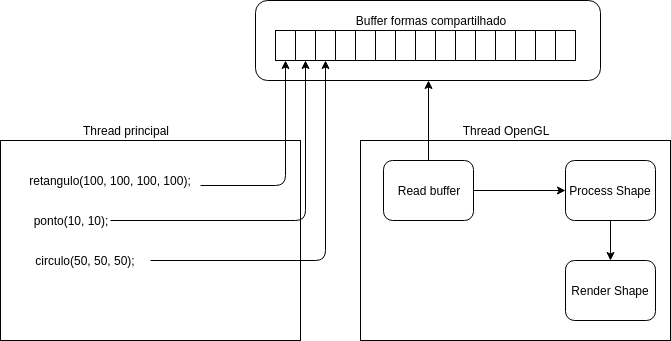
\includegraphics[scale=0.65]{images/basic_architecture.png}
  \caption{Arquitetura proposta para a biblioteca}
  \label{fig:arquitetura_proposta}
\end{figure}

A biblioteca gráfica dispõe da API abaixo:

\begin{itemize}
    \item void inicializarBiblioteca(int largura, int altura);
    \item void limparTela();
    
    \item void desfazerUltimaForma();
    \item void refazerUltimaForma();
    
    \item void definirCor(int vermelho, int verde, int azul);
    \item int* obterCor();
    
    \item void definirEspessura(int espessura);
    \item int obterEspessura();

    \item void poligono(int numeroDeVertices, GLfloat* posicoes);
    \item void ponto(int posX, int posY);
    \item void triangulo(int posX1, int posY1, int posX2, int posY2, int posX3, int posY3);
    \item void retangulo(int posX, int posY, int largura, int altura);
    \item void quadrado(int posX, int posY, int tamanhoLado);
    \item void poligonoRegular(int posX, int posY, int raio, int faces);
    \item void circulo(int posX, int posY, int raio);
    \item void pentagono(int posX, int posY, int raio);
    \item void hexagono(int posX, int posY, int raio);
    \item void decagono(int posX, int posY, int raio);
    \item void dodecagono(int posX, int posY, int raio);
    \item void linha(int posX1, int posY1, int posX2, int posY2);
    
    \item void pausar(int time);
\end{itemize}

As seções seguintes descrevem cada item da API bem como seus protótipos e o significado de cada parâmetro de entrada.

\subsubsection{Iniciando a biblioteca}
Apesar de não ter que gerenciar diretamente a janela e o laço de repetição de renderização do OpenGL manualmente, ainda é necessário inicializar a biblioteca manualmente, para disparar a \textit{thread} secundária, responsável pela renderização dos objetos, e a criação da janela onde serão renderizadas os objetos.

A função que inicializa a biblioteca tem o seguinte protótipo:

\begin{minted}{c}
void inicializarBiblioteca(int largura, int altura);
\end{minted}

Os parâmetros de entrada são:

\begin{itemize}
    \item int largura - a largura do tamanho da janela a ser criada.
    \item int altura -  altura do tamanho da janela a ser criada.
\end{itemize}

O exemplo abaixo mostra como inicializar a biblioteca em uma aplicação C e o resultado pode ser observado na Figura~\ref{fig:exemplo_initWindow}:
\begin{listing}[ht]
\begin{minted}{c}
#include <stdio.h>
#include <graphics.h>

int main() {
    inicializarBiblioteca(800, 600);

    retangulo(0, 0, 200, 100);
    limparTela();

    getchar();
    return 0;
}
\end{minted}
\caption{Inicializando a biblioteca}
\label{lst:inicializando_biblioteca}
\end{listing}

\begin{figure}[!htbp]
  \centering
  \includegraphics[scale=0.7]{images/exemplo_initWindow.JPG}
  \caption{Exemplo inicialização da biblioteca}
  \label{fig:exemplo_initWindow}
\end{figure}

\subsubsection{Limpando a tela}
Uma das funcionalidades propostas é que a janela seja limpa, removendo assim todos os objetos renderizados e reiniciando a janela para seu estado inicial.

A função que limpa a janela já foi utilizada anteriormente e pode ser encontrada no Exemplo~\ref{lst:inicializando_biblioteca}.

\subsubsection{Desfazer último desenho}
Em uma aplicação, é comum se arrepender de sua última ação e portanto, querer desfaze-la. A biblioteca aqui implementada possui uma função específica para esta ação. Ela pode ser utilizada múltiplas vezes e a cada vez um objeto é removido da tela.

A função que desfaz o último desenho tem o seguinte protótipo:

\begin{minted}{c}
void desfazerUltimaForma();
\end{minted}

\subsubsection{Refazer o último desenho}
Refazer o último desenho é uma opção da mesma forma que desfazer o último desenho. Sendo assim, é possível se arrepender e desfazer a opção de desfazer. A cada vez que a função for chamada, um desenho será restaurado. A ordem de restauração é baseada na estrutura de dados pilha, portanto o último objeto removido será o primeiro objeto restaurado. Essa função só pode ser executa caso invocada imediatamente após a função de desfazer, pois caso seja inserida um novo objeto após ter desfeito o último desenho, a pilha de ações será descartada.

A função que refaz o último desenho tem o seguinte protótipo:

\begin{minted}{c}
void refazerUltimaForma();
\end{minted}

\subsubsection{Alterar a cor de preenchimento de um objeto} \label{api_definirCor}
A grande maioria, senão todas, as biblioteca citadas nos trabalhos correlatos permitem a definição de uma cor de preenchimento para o objeto a ser desenhado.

A função que permite alterar a cor de um objeto tem o seguinte protótipo:

\begin{minted}{c}
void definirCor(int vermelho, int verde, int azul);
\end{minted}

Os parâmetros de entrada são:

\begin{itemize}
    \item int vermelho - um inteiro de 0 a 255 representando a tonalidade de vermelho do padrão RGB.
    \item int verde - um inteiro de 0 a 255 representando a tonalidade de verde do padrão RGB.
    \item int azul - um inteiro de 0 a 255 representando a tonalidade de azul do padrão RGB.
\end{itemize}

\subsubsection{Obter a cor de preenchimento do objeto}
Assim como podemos definir a cor de preenchimento de um objeto, também é possível obtermos a cor de preenchimento atual. Esta função se faz útil quando, por exemplo, queremos criar um objeto de uma nova cor mas queremos manter a cor antiga, porém não é conhecido a cor de preenchimento atual. Assim como visto no item~\ref{api_definirCor}, como a função \textit{definirCor} recebe 3 argumentos de entrada, a saída é um ponteiro representando um array de inteiros de tamanho 3, representando as cores RGB.

A função que obtém a cor atual de uma forma tem o seguinte protótipo:

\begin{minted}{c}
int* obterCor();
\end{minted}

A saída do método é um ponteiro para um array contendo 3 posições e seus valores são descritos conforme a lista abaixo:

\begin{itemize}
    \item int cor[0] - um inteiro de 0 a 255 representando a tonalidade de vermelho do padrão RGB.
    \item int cor[1] - um inteiro de 0 a 255 representando a tonalidade de verde do padrão RGB.
    \item int cor[2] - um inteiro de 0 a 255 representando a tonalidade de azul do padrão RGB.
\end{itemize}

O exemplo abaixo mostra como obter a cor atual de uma forma em uma aplicação C:

\begin{minted}{c}
#include <stdio.h>
#include <graphics.h>

int main() {
    inicializarBiblioteca(800, 600);

    definirCor(255, 0, 127);
    retangulo(0, 0, 200, 100);

    int* corAtual = obterCor();

    getchar();
    return 0;
}
\end{minted}

\subsubsection{Definindo o tamanho de um objeto}
Alguns objetos podem ter seu tamanho alterado. Para que tenha efeito, a função \textit{definirTamanho} deve ser invocada anteriormente a uma função de desenho de forma. Após chamado o método, todos os objetos desenhados após a chamada serão desenhados com o novo tamanho definido. Atualmente apenas o objeto \textit{ponto} pode ter seu tamanho alterado.

A função que define o tamanho de uma forma tem o seguinte protótipo:

\begin{minted}{c}
void definirTamanho(int tamanho);
\end{minted}

O exemplo abaixo mostra como definir o tamanho de uma forma em uma aplicação C:

\begin{minted}{c}
#include <stdio.h>
#include <graphics.h>

int main() {
    inicializarBiblioteca(800, 600);

    definirTamanho(50);
    ponto(100, 100);

    getchar();
    return 0;
}
\end{minted}

\subsubsection{Obtendo o tamanho de um objeto}
Da mesma forma que é possível definir o tamanho de um objeto, esta função permite obter o valor atual do tamanho de desenho de objetos. Esta função é útil quando se quer desenhar um objeto em novo tamanho e deseja retornar o tamanho anterior para os próximos objetos e não existe a informação de qual o valor atual do tamanho da forma.

A função de como obter o tamanho atual de uma forma tem o seguinte protótipo:

\begin{minted}{c}
int obterTamanho();
\end{minted}

O exemplo abaixo mostra como obter o tamanho atual de uma forma em uma aplicação C:

\begin{minted}{c}
#include <stdio.h>
#include <graphics.h>

int main() {
    inicializarBiblioteca(800, 600);

    definirTamanho(50);
    ponto(100, 100);

    int tamanhoAtual = obterTamanho();

    getchar();
    return 0;
}
\end{minted}

\subsubsection{Desenhando um polígono}
Um polígono é uma figura geométrica composta por 3 ou mais vértices. Um polígono pode ser desenhado de forma livre e a função que desenha um polígono tem o seguinte protótipo:

\begin{minted}{c}
void poligono(int numeroDeVertices, GLfloat* posicoes);
\end{minted}

Os parâmetros de entrada são:

\begin{itemize}
    \item int numeroDeVertices - número de vértices que o seu polígono possui
    \item GLfloat* posicoes - um array contendo as posições de cada vértice. O array deve possuir um tamanho par definido pela fórmula \(tamanho = 2 \times numeroDeVertices \), pois as posições pares representam as posições X dos vértices e as posições ímpares representam as posições Y, par a par. Os pares devem ser definidos sequencialmente. Para desenhar um triângulo, seria então necessário um array de 6 posições. Utilizando um triângulo como exemplo, vamos utilizar os pontos (0, 0), (200, 0) e (100, 200). O array de posições então seria \textit{GLfloat posicoes[6] = \{0, 0, 200, 0, 100, 200\};}.
\end{itemize}

O exemplo abaixo mostra como desenhas um polígono em uma aplicação C:

\begin{minted}{c}
#include <stdio.h>
#include <stdlib.h>
#include <graphics.h>

int main() {
    inicializarBiblioteca(800, 600);

    GLfloat posicoes[] = {
        320, 100,
        400, 300,
        800, 50,
        520, 10,
        340, 40
    };
    poligono(5, posicoes);

    getchar();
    return 0;
}
\end{minted}

\subsubsection{Desenhando um ponto}
A função que desenha um ponto tem o seguinte protótipo:

\begin{minted}{c}
void ponto(int posX, int posY);
\end{minted}

Os parâmetros de entrada são:

\begin{itemize}
    \item int posX - a posição X do ponto.
    \item int posY - a posição Y do ponto.
\end{itemize}

\subsubsection{Desenhando um triângulo}
Triângulos são uma das formas mais básicas e utilizadas, pois todos os polígonos convexos pode ser decompostos em vários triângulos. A função que desenha um triângulo tem o seguinte protótipo:

\begin{minted}{c}
void triangulo(
    int posX1, int posY1,
    int posX2, int posY2,
    int posX3, int posY3
);
\end{minted}

Os parâmetros de entrada são:

\begin{itemize}
    \item int posX1 - a posição X da vértice 1 do triângulo.
    \item int posY1 - a posição Y da vértice 1 do triângulo.

    \item int posX2 - a posição X da vértice 2 do triângulo.
    \item int posY2 - a posição Y da vértice 2 do triângulo.

    \item int posX3 - a posição X da vértice 3 do triângulo.
    \item int posY3 - a posição Y da vértice 3 do triângulo.
\end{itemize}

\subsubsection{Desenhando um retângulo}
Retângulos são formas geométricas que possuem 4 ângulos retos. Por serem uma das mais básicas formas, são bastante utilizados

A função que desenha um retângulo tem o seguinte protótipo:

\begin{minted}{c}
void retangulo(int posX, int posY, int largura, int altura);
\end{minted}

Os parâmetros de entrada são:

\begin{itemize}
    \item int posX - posição X do retângulo. Representa o vértice inferior esquerdo do retângulo.
    \item int posY - posição y do retângulo. Representa o vértice inferior esquerdo do retângulo.
    \item int altura - altura do triângulo.
    \item int largura - largura do triângulo.
\end{itemize}

\subsubsection{Desenhando um quadrado}
Um quadrado é um polígono considerado especial, pois trata-se de um retângulo que possui largura e altura de mesmo tamanho.

A função que desenha um quadrado tem o seguinte protótipo:

\begin{minted}{c}
void quadrado(int posX, int posY, int tamanhoLado);
\end{minted}

Os parâmetros de entrada são:

\begin{itemize}
    \item int posX - posição X do quadrado. Representa o vértice inferior esquerdo do quadrado.
    \item int posY - posição Y do quadrado. Representa o vértice inferior esquerdo do quadrado.
    \item int tamanhoLado - tamanho do lado do quadrado.
\end{itemize}

\subsubsection{Desenhando um polígono regular}
Um polígono regular é um polígono convexo com \textit{n} faces onde cada face possui o mesmo tamanho e todos os ângulos internos são iguais. Alguns exemplos de polígonos regulares são triângulos retângulos, quadrados, pentágonos, hexágonos, dentre outros. Algumas dessas formas você pode ver na Figura~\ref{fig:poligonos_regulares}.

\begin{figure}[htbp]
  \centering
  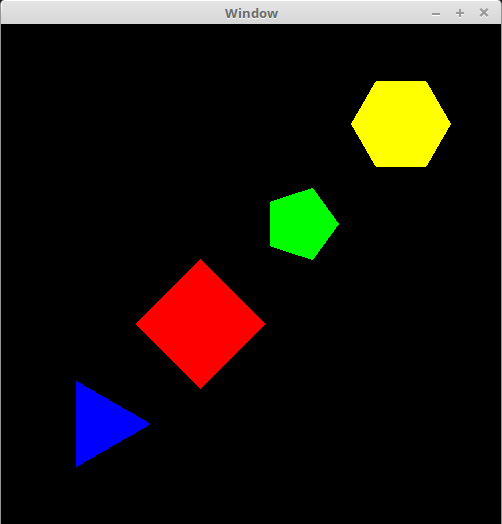
\includegraphics[scale=0.51]{images/poligonos_regulares.png}
  \caption{Exemplos de polígonos regulares: Triângulo, quadrado, pentágono e hexágono}
  \label{fig:poligonos_regulares}
\end{figure}

Segundo \citeonline{PoligonoConvexos:BrasilEscola}, ``um polígono é convexo quando todos os pontos de um segmento de reta que possui as extremidades no interior do polígono também estão dentro dele. Sendo assim, se for possível encontrar pelo menos um segmento de reta que possui as extremidades dentro do polígono e, ao mesmo tempo, um ponto fora dele, esse polígono não será convexo''.

A função que desenha um polígono regular tem o seguinte protótipo:

\begin{minted}{c}
void poligonoRegular(int posX, int posY, int raio, int faces);
\end{minted}

Os parâmetros de entrada são:

\begin{itemize}
    \item int posX - posição X onde do polígono regular. Representa o centro de onde será desenhado o objeto.
    \item int posY - posição Y onde do polígono regular. Representa o centro de onde será desenhado o objeto.
    \item int raio - tamanho do raio que do polígono regular.
    \item int faces - o número de faces que do polígono regular.
\end{itemize}

O exemplo abaixo mostra como desenhar um polígono regular azul em uma aplicação C:

\begin{minted}{c}
#include <stdio.h>
#include <stdlib.h>
#include <graphics.h>

int main() {
    inicializarBiblioteca(800, 600);

    definirCor(0, 0, 255);
    poligonoRegular(300, 300, 100, 7);

    getchar();
    return 0;
}
\end{minted}

\subsubsection{Desenhando um círculo}
O círculo é uma forma geométrica que possui virtualmente infinitos vértices.

A função que desenha um círculo tem o seguinte protótipo:

\begin{minted}{c}
void circulo(int posX, int posY, int raio);
\end{minted}

Os parâmetros de entrada são:

\begin{itemize}
    \item int posX - posição X do centro do círculo.
    \item int posY - posição Y do centro do círculo.
    \item int raio - raio do círculo.
\end{itemize}

\subsubsection{Desenhando um pentágono}
Um pentágono é um polígono regular composto por 5 vértices.

A função que desenha um pentágono tem o seguinte protótipo:

\begin{minted}{c}
void pentagono(int posX, int posY, int raio);
\end{minted}

Os parâmetros de entrada são:

\begin{itemize}
    \item int posX - posição X do centro do pentágono.
    \item int posY - posição Y do centro do pentágono.
    \item int raio - raio do pentágono.
\end{itemize}

\subsubsection{Desenhando uma linha}
Dado 2 pontos A e B, uma linha é um segmento de reta que liga os pontos A e B.

A função que desenha uma linha tem o seguinte protótipo:

\begin{minted}{c}
void linha(int posX1, int posY1, int posX2, int posY2);
\end{minted}

Os parâmetros de entrada são:

\begin{itemize}
    \item int posX1 - posição do X1 da linha.
    \item int posY1 - posição do Y1 da linha.
    \item int posX2 - posição do X2 da linha.
    \item int posY2 - posição do Y2 da linha.
\end{itemize}

O exemplo abaixo mostra como desenhar uma linha que corta a janela de desenho verticalmente em uma aplicação C:

\begin{minted}{c}
#include <stdio.h>
#include <graphics.h>

int main() {
    inicializarBiblioteca(1366, 768);

    linha(
        0, 0,
        1366, 768
    );

    getchar();
    return 0;
}
\end{minted}

\section{Estado Atual do Desenvolvimento}
No estado atual do desenvolvimento todas as funcionalidades previstas foram implementadas e funcionam de forma portável e multiplataforma. Todas as formas implementadas podem ser observadas na Figura~\ref{fig:todas_formas}.

\begin{figure}[htbp]
  \centering
  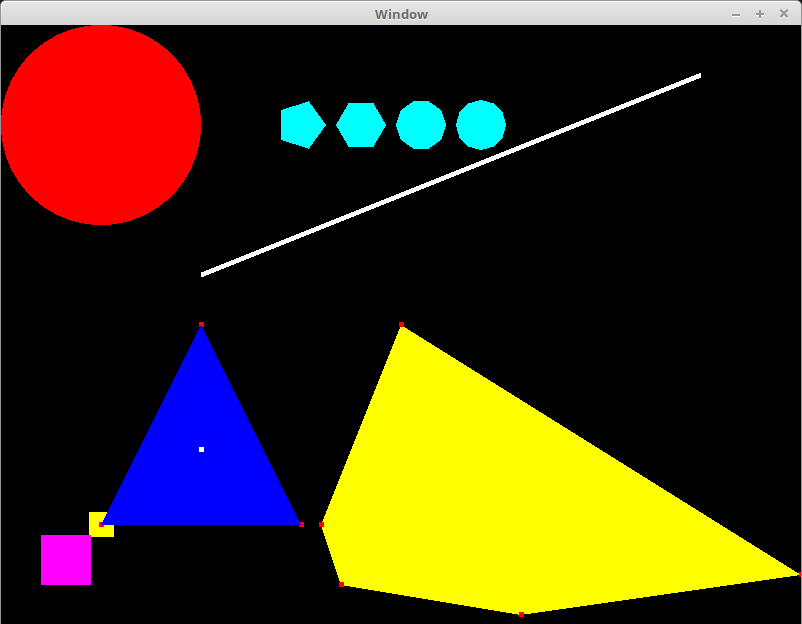
\includegraphics[scale=0.51]{images/objetos_disponiveis.png}
  \caption{Exemplo: Todas as formas implementadas}
  \label{fig:todas_formas}
\end{figure}

Como todas as funcionalidades foram implementadas, os usuário são capazes de desenhar objetos e cenas que sejam baseados nas formas implementadas. Um exemplo de uso mostrando como desenhar um relógio funcional utilizando a biblioteca desenvolvida neste projeto, utilizando linguagem de programação C, pode ser visto na Figura~\ref{fig:exemplo_relogio}.

\begin{figure}[htbp]
  \centering
  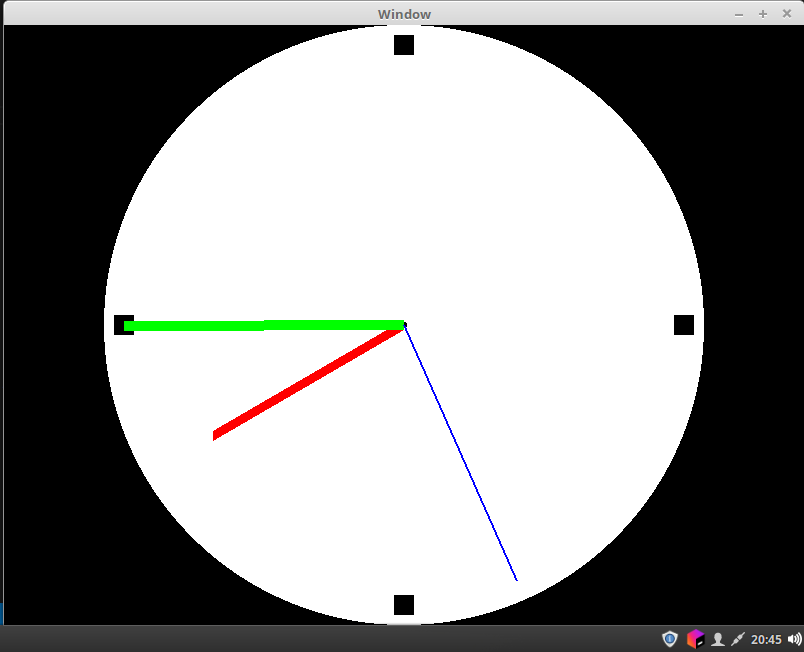
\includegraphics[scale=0.51]{images/exemplo_relogio.png}
  \caption{Exemplo: Relógio analógico}
  \label{fig:exemplo_relogio}
\end{figure}

Um ponto muito importante é a ausência de testes automatizados. Toda alteração em softwares que não possuem testes automatizados correm o risco de quebrar a compatibilidade com versões anteriores ou em evoluções de manutenção corretiva. Logo, os testes devem ser realizados pelo usuário, no projeto que estiver sendo desenvolvido utilizando esta biblioteca.

O código-fonte da biblioteca descrita neste projeto, bem como a documentação, o guia de uso e alguns exemplos de utilização podem ser encontrados na lista abaixo:

\begin{itemize}
    \item \url{https://github.com/williamokano/tcc/tree/master/src}: Contém o código-fonte da biblioteca. Este código deve ser compilado para gerar o arquivo biblioteca a ser importado em seu projeto;
    \item \url{https://github.com/williamokano/tcc/tree/master/headers}: Contém os arquivos cabeçalhos para utilização em conjunto com a biblioteca gráfica;
    \item \url{https://github.com/williamokano/tcc/tree/master/documentacao}: Contém os arquivos de documentação da biblioteca, onde é explicado cada função e seus parâmetros;
    \item \url{https://github.com/williamokano/tcc/tree/master/guia}: Contém um guia ilustrado mostrando como utilizar a biblioteca em ambientes Windows e Linux;
    \item \url{https://github.com/williamokano/tcc/tree/master/exemplos}: Contém alguns exemplos criados utilizando a biblioteca. Os exemplos incluem, mas não se limitam a, uma figura se movendo pela tela, um relógio, desenhos na tela utilizando entradas fornecidas pelo usuário.
\end{itemize}

\chapter{Considerações Finais}

\section{Trabalhos Futuros}
Como trabalho futuro, um dos principais pontos a ser trabalho é o uso da biblioteca aqui descrita em salas de aula. Elaborar algum método de avaliação capaz de medir a assimilação do conteúdo pela utilização da biblioteca e verificar se ela realmente gera os resultados esperados.

Como dito na Seção~\ref{lbl:linguagem_programao_c}, os dados obtidos para esta pesquisa foram provenientes de um grupo de programação online. Assim, uma sugestão para trabalhos futuros seria refazer esta mesma pesquisa utilizando dados de faculdades e universidades brasileiras de ensino de Ciência da Computação, Sistemas de Informação ou cursos similares. Com esta abordagem, pode-se obter valores mais precisos sobre a real utilização da linguagem C como linguagem de cursos introdutórios de programação.

Outro ponto interessante seria a adição de novas funcionalidades de desenho, como elipses, arcos, linhas curvas e textos. Com essas novas funcionalidades o usuário teria um novo leque de funcionalidades como, por exemplo, a criação, de forma bem simplificada, de gráficos de barras e de linhas. A habilidade de poder se expressar por texto, além das formas geométricas, seria uma excelente adição para os próximos trabalhos.

Com o intuito de deixar a biblioteca mais segura, o desenvolvimento de testes automatizados podem ser incluídos, a fim de garantir que a compatibilidade não seja quebrada entre versões ou que, caso isso ocorra, que tenha sido proposital.

Outra possibilidade seria evoluir a biblioteca de forma que deixe ser apenas para formas geométricas e possa começar a importar recursos externos, como por exemplo imagens e sons. Com essa evolução, a biblioteca ficaria mais dinâmica e possibilitaria um novo leque de possibilidades ao usuário, como o desenvolvimento de jogos simples.

\section{Dificuldades Encontradas}
Inicialmente uma das dificuldades encontradas foi conseguir compilar a biblioteca de uma forma que fosse simples de utilizar tanto no sistema operacional Linux quanto no Windows. A primeira abordagem foi utilizar o \citeonline{CMake:About}, pois ele possui o mesmo suporte de macros que a linguagem C, portanto deveria ser fácil a compilação multiplataforma. Entretanto, algumas macros, como a \#\_\_WIN32, que indica se o sistema operacional é Windows, nem sempre é adicionada no momento da compilação. Com isso, a possibilidade de utilizar CMake como ferramenta de compilação foi excluída.

A ideia inicial deste projeto era criar uma biblioteca que, além de ser simples, não necessita-se de outras bibliotecas complementares para o gerenciamento de janelas e contextos do OpenGL. Entretanto, mostrou-se muito difícil realizar essas implementações, pois o sistema de janelas dos sistemas operacionais Windows e Linux são completamente diferentes. No sistema operacional Windows, para o gerenciamento de janelas, é utilizado a API do Windows, através da biblioteca win32.dll. Já no sistema operacional Linux, todo o sistema de gerencimanto de janelas é realizado através da biblioteca X11. Essa gestão de janelas é muito complexa, mesmo quando estamos desenvolvendo exclusivamente para um sistema operacional, portanto foi utilizado a biblioteca GLFW para gerenciar as janelas de forma portável e multiplataforma.

Mesmo utilizando a biblioteca GLFW, a compilação multiplataforma não foi direta. No sistema operacional Windows a biblioteca GLFW é compilada antes da biblioteca descrita neste trabalho, e logo após é realizado o link estático entre as duas bibliotecas. A estratégia utilizada no sistema operacional Linux foi instalar a biblioteca GLFW através de um gerenciador de pacotes e então realizar o link compartilhado no ato da compilação da biblioteca deste projeto.

Outra dificuldade encontrada foi a compilação da biblioteca TinyCThread no sistema operacional Windows. Inicialmente o compilador utilizado era o mingw, um kit de ferramentas para Windows contento o compilador GCC e algumas bibliotecas previamente instalas. Este compilador foi instalado automaticamente junto com a IDE \citeonline{CodeBlocks:About}. Entretanto a versão instalada com essa IDE não é suportada pela TinyCThread. A versão recomendada do mingw para compilar a biblioteca TinyCThread no sistema operacional Windows é a versão mingw64. Após instalar essa versão, o problema foi sanado.

%\chapter{Desenvolvimento}
%Um ou mais capítulos (por exemplo um para testes)

% ---
% Conclusão
% ---
\chapter*[Conclusão]{Conclusão}
\addcontentsline{toc}{chapter}{Conclusão}
%TCC:
Este trabalho apresentou uma biblioteca para auxiliar o aluno a assimilar melhor os códigos ensinados em cursos introdutórios de programação, utilizando técnicas de visualização. Os problemas causados pela falta de assimilação dos conceitos ensinados nos cursos de programação pode levar o aluno a ter um atraso em outras disciplinas onde o conhecimento de programação é requisito, como por exemplo, na disciplina de estrutura de dados. Além do mais, alunos que não conseguem assimilar o conhecimento introdutório de programação podem acabar se frustando e abandonando o curso, aumentando assim o índice de evasão.

Para poder realizar este trabalho, foi necessário uma base teórica multidisciplinar, onde a maioria do conhecimento foi obtido através de disciplinas oferecidas pelo curso de Sistemas de Informação. As disciplinas de Modelagem de Software, Engenharia de Software, Sistemas Operacionais e Estrutura de Dados foram primordiais para que fosse desenvolvida uma arquitetura simples e eficiente. Conceitos como \textit{multi threading}, \textit{locks} de exclusão mútua, ensinados em Sistemas Operacionais, foram essenciais para o desenvolvimento desta biblioteca. Os conhecimentos ensinados em Estrutura de Dados, como listas e pilhas, também foram utilizados para o desenvolvimento da biblioteca, seja para o armazenamento dos objetos em um \textit{buffer}, que é uma lista, ou então a utilização de uma pilha, para que pudesse ser implementado o conceito de desfazer e refazer uma ação. Além do mais, os conhecimentos obtidos em Modelagem de Software e Engenharia de Software foram de grande ajuda para que fosse possível entender o problema e modelar a arquitetura para que fosse obtida uma API simples e de fácil utilização.

% ----------------------------------------------------------
% ELEMENTOS PÓS-TEXTUAIS
% ----------------------------------------------------------
\postextual

%\nocite{babel}
% ----------------------------------------------------------
% Referências bibliográficas
% ----------------------------------------------------------
\bibliography{referencias}


%% ----------------------------------------------------------
%% Apêndices TCC: só mantenha se for pertinente.
%% ----------------------------------------------------------

\iffalse
% ---
% Inicia os apêndices
% ---
\begin{apendicesenv}

% Imprime uma página indicando o início dos apêndices
\partapendices
% ----------------------------------------------------------
\chapter{Quisque libero justo}
% ----------------------------------------------------------

\lipsum[50]

% ----------------------------------------------------------
\chapter{Coisas que fiz e que achei interessante mas não tanto para entrar no corpo do texto}
% ----------------------------------------------------------
\lipsum[55-57]
\end{apendicesenv}
\fi
% ---


% ----------------------------------------------------------
% Anexos %TCC: so mantenha se pertinente.
% ----------------------------------------------------------

\iffalse
% ---
% Inicia os anexos
% ---
\begin{anexosenv}

% Imprime uma página indicando o início dos anexos
\partanexos
% ---
\chapter{Eu sempre quis aprender latim}
% ---
\lipsum[30]

% ---
\chapter{Coisas que eu não fiz mas que achei interessante o suficiente para colocar aqui}
% ---

\lipsum[31]

% ---
\chapter{Fusce facilisis lacinia dui}
% ---

\lipsum[32]
\end{anexosenv}
\fi

%---------------------------------------------------------------------
% INDICE REMISSIVO
%---------------------------------------------------------------------

\printindex



\end{document}
